\documentclass[12pt]{article}
\usepackage{graphicx}
\usepackage{cite}
\usepackage{geometry}
\usepackage{hyperref}
\usepackage{natbib}
\usepackage{caption}
\bibliographystyle{ieeetr}
\setcitestyle{super,open={[},close={]}}

\usepackage{color}
\definecolor{darkred}{rgb}{0.6,0.0,0.0}
\definecolor{darkgreen}{rgb}{0,0.50,0}
\definecolor{lightblue}{rgb}{0.0,0.42,0.91}
\definecolor{orange}{rgb}{0.99,0.48,0.13}
\definecolor{grass}{rgb}{0.18,0.80,0.18}
\definecolor{pink}{rgb}{0.97,0.15,0.45}

\usepackage{xcolor}
\definecolor{codegray}{rgb}{0.85, 0.85, 0.85}

\usepackage{listings}
\lstset{
  aboveskip=1em,
  breaklines=true,
  abovecaptionskip=-6pt,
  captionpos=b,
  escapeinside={\%*}{*)},
  frame=single
}

\lstdefinestyle{colored}{
  basicstyle=\ttfamily,
  backgroundcolor=\color{white},
  commentstyle=\color{green}\itshape,
  keywordstyle=\color{blue}\bfseries\itshape,
  stringstyle=\color{red},
}

\lstdefinelanguage{PythonPlus}[]{Python}{
  morekeywords=[1]{,as,assert,nonlocal,with,yield,self,True,False,None,}
  morekeywords=[2]{,__init__,__add__,__mul__,__div__,__sub__,__call__,__getitem__,__setitem__,__eq__,__ne__,__nonzero__,__rmul__,__radd__,__repr__,__str__,__get__,__truediv__,__pow__,__name__,__future__,__all__,}, % magic methods
  morekeywords=[3]{,object,type,isinstance,copy,deepcopy,zip,enumerate,reversed,list,set,len,dict,tuple,range,xrange,append,execfile,real,imag,reduce,str,repr,}, % common functions
  morekeywords=[4]{,Exception,NameError,IndexError,SyntaxError,TypeError,ValueError,OverflowError,ZeroDivisionError,}, % errors
  morekeywords=[5]{,ode,fsolve,sqrt,exp,sin,cos,arctan,arctan2,arccos,pi, array,norm,solve,dot,arange,isscalar,max,sum,flatten,shape,reshape,find,any,all,abs,plot,linspace,legend,quad,polyval,polyfit,hstack,concatenate,vstack,column_stack,empty,zeros,ones,rand,vander,grid,pcolor,eig,eigs,eigvals,svd,qr,tan,det,logspace,roll,min,mean,cumsum,cumprod,diff,vectorize,lstsq,cla,eye,xlabel,ylabel,squeeze,}, % numpy / math
}

\lstdefinelanguage{PyBrIM}[]{PythonPlus}{
  emph={d,E,a,Fc28,Fy,Fu,D,des,supplier,Material,Rectangle,PyElmt},
}

\lstdefinestyle{colorEX}{
  basicstyle=\ttfamily,
  backgroundcolor=\color{white},
  commentstyle=\color{darkgreen}\slshape,
  keywordstyle=\color{blue}\bfseries\itshape,
  keywordstyle=[2]\color{blue}\bfseries,
  keywordstyle=[3]\color{grass},
  keywordstyle=[4]\color{red},
  keywordstyle=[5]\color{orange},
  stringstyle=\color{darkred},
  emphstyle=\color{pink}\underbar,
}

\geometry{margin=1in}

\begin{document}
\begin{center}
\LARGE
\textbf{Apache Openwhisk} \vspace{10pt}\\
\Large
\textbf{Distributed Software Systems, 2024/25} \vspace{10pt}\\
\large
\textbf{Davide De Rosa}
\end{center}

\section{Introduction to Serverless Computing}
Scalability and Elasticity are essential features of Cloud Computing, yet even after a decade, they remain inaccessible for many cloud users. Although cloud computing has freed developers from managing physical infrastructure, it still requires oversight of virtual resources for software deployments. These limitations, combined with the shift toward containers and microservices in enterprise application architectures, have given rise to a new deployment paradigm known as \textbf{Serverless Cloud Computing}\cite{banaei2022etas}.\vspace{14pt}\\
Over the past decade, cloud platform hosting has evolved significantly\cite{djemame2020open}:
\begin{itemize}
    \item Initially, organizations purchased or rented physical servers to run applications, incurring costs for both the hardware and its maintenance.
    \item This shifted with the adoption of \textbf{virtualization}, which allowed a single physical server to function as multiple software-defined Virtual Machines (VMs), enhancing flexibility and resource utilization. \textbf{Containerization} emerged as a further refinement, combining aspects of virtualization with configuration management.
    \item The introduction of \textbf{Platform-as-a-Service} (\textbf{PaaS}) took abstraction further, freeing users from managing servers and deployment processes.
    \item The latest advancement, serverless computing, builds on \textit{PaaS} by enabling deployment of small code fragments that can autonomously scale, supporting the creation of self-scaling applications.
\end{itemize}
Serverless computing, also called \textbf{Function as a Service} (\textbf{FaaS}), completely separates backend infrastructure management from application development, hiding server maintenance responsibilities from users. In serverless computing, the cloud provider handles \textit{server management}, \textit{function execution}, \textit{capacity planning}, \textit{resource allocation}, \textit{task scheduling}, \textit{scalability}, \textit{deployment}, \textit{operational monitoring}, and \textit{security updates}. This model implements \textbf{event-driven programming}, where applications utilize \textbf{small}, \textbf{stateless functions} (or handlers) that are \textbf{triggered by events}.\\
Users simply upload code, trigger stateless functions through events, and \textbf{pay only for the actual runtime of their code}.\vspace{14pt}\\
Delegating server management to cloud providers presents both benefits and challenges for \textit{providers} and \textit{users}.\vspace{14pt}\\
For \textbf{users}, serverless computing eliminates the need for server management while offering a simplified programming model that abstracts many operational concerns. Features like autoscaling and scaling to zero enable genuine pay-as-you-go billing.\\
However, challenges remain, including limited support for different programming languages and libraries, state management, monitoring, debugging, and execution time constraints.\vspace{14pt}\\
For \textbf{cloud providers}, serverless computing offers new opportunities by allowing full resource control and operational cost reduction through optimized resource management.\\
At the same time, providers face significant challenges such as cold starts (the delay in starting a new function instance), scheduling policies, scaling, performance prediction, dynamic resource provisioning, I/O bottlenecks, communication delays due to slow storage, pricing models, and issues around security and privacy.\cite{banaei2022etas}

\section{Serverless Architecture}
Serverless computing has become a key model for developing and deploying cloud applications, offering a zero-administration approach by fully decoupling backend infrastructure management from application development. In this model, applications are composed of small, stateless functions or handlers that operate independently and execute in response to specific events. Cloud providers run these handlers in isolated sandboxes, such as \textbf{containers}, allowing for both \textbf{secure isolation} and \textbf{efficient autoscaling}, while enabling a genuine pay-as-you-go billing model.\vspace{14pt}\\
The architecture of a serverless platform is illustrated in Fig. 1. In this setup, the serverless platform receives an event sent via HTTP or another cloud-based source. Internally, the platform includes an event queue, a dispatcher, and worker nodes. Upon receiving a request, the system identifies the appropriate function(s) to handle the event. The dispatcher then routes the request to a worker node, retrieving the necessary function code from a database.\vspace{14pt}\\
The worker node executes the function(s), launching one or more instances depending on the request volume and available resources. If resources are sufficient, function instances (typically run in containers) are launched with restricted resources to carry out the task. If resources are limited, the function request is queued until resources become available.\vspace{10pt}\\
\begin{center}
    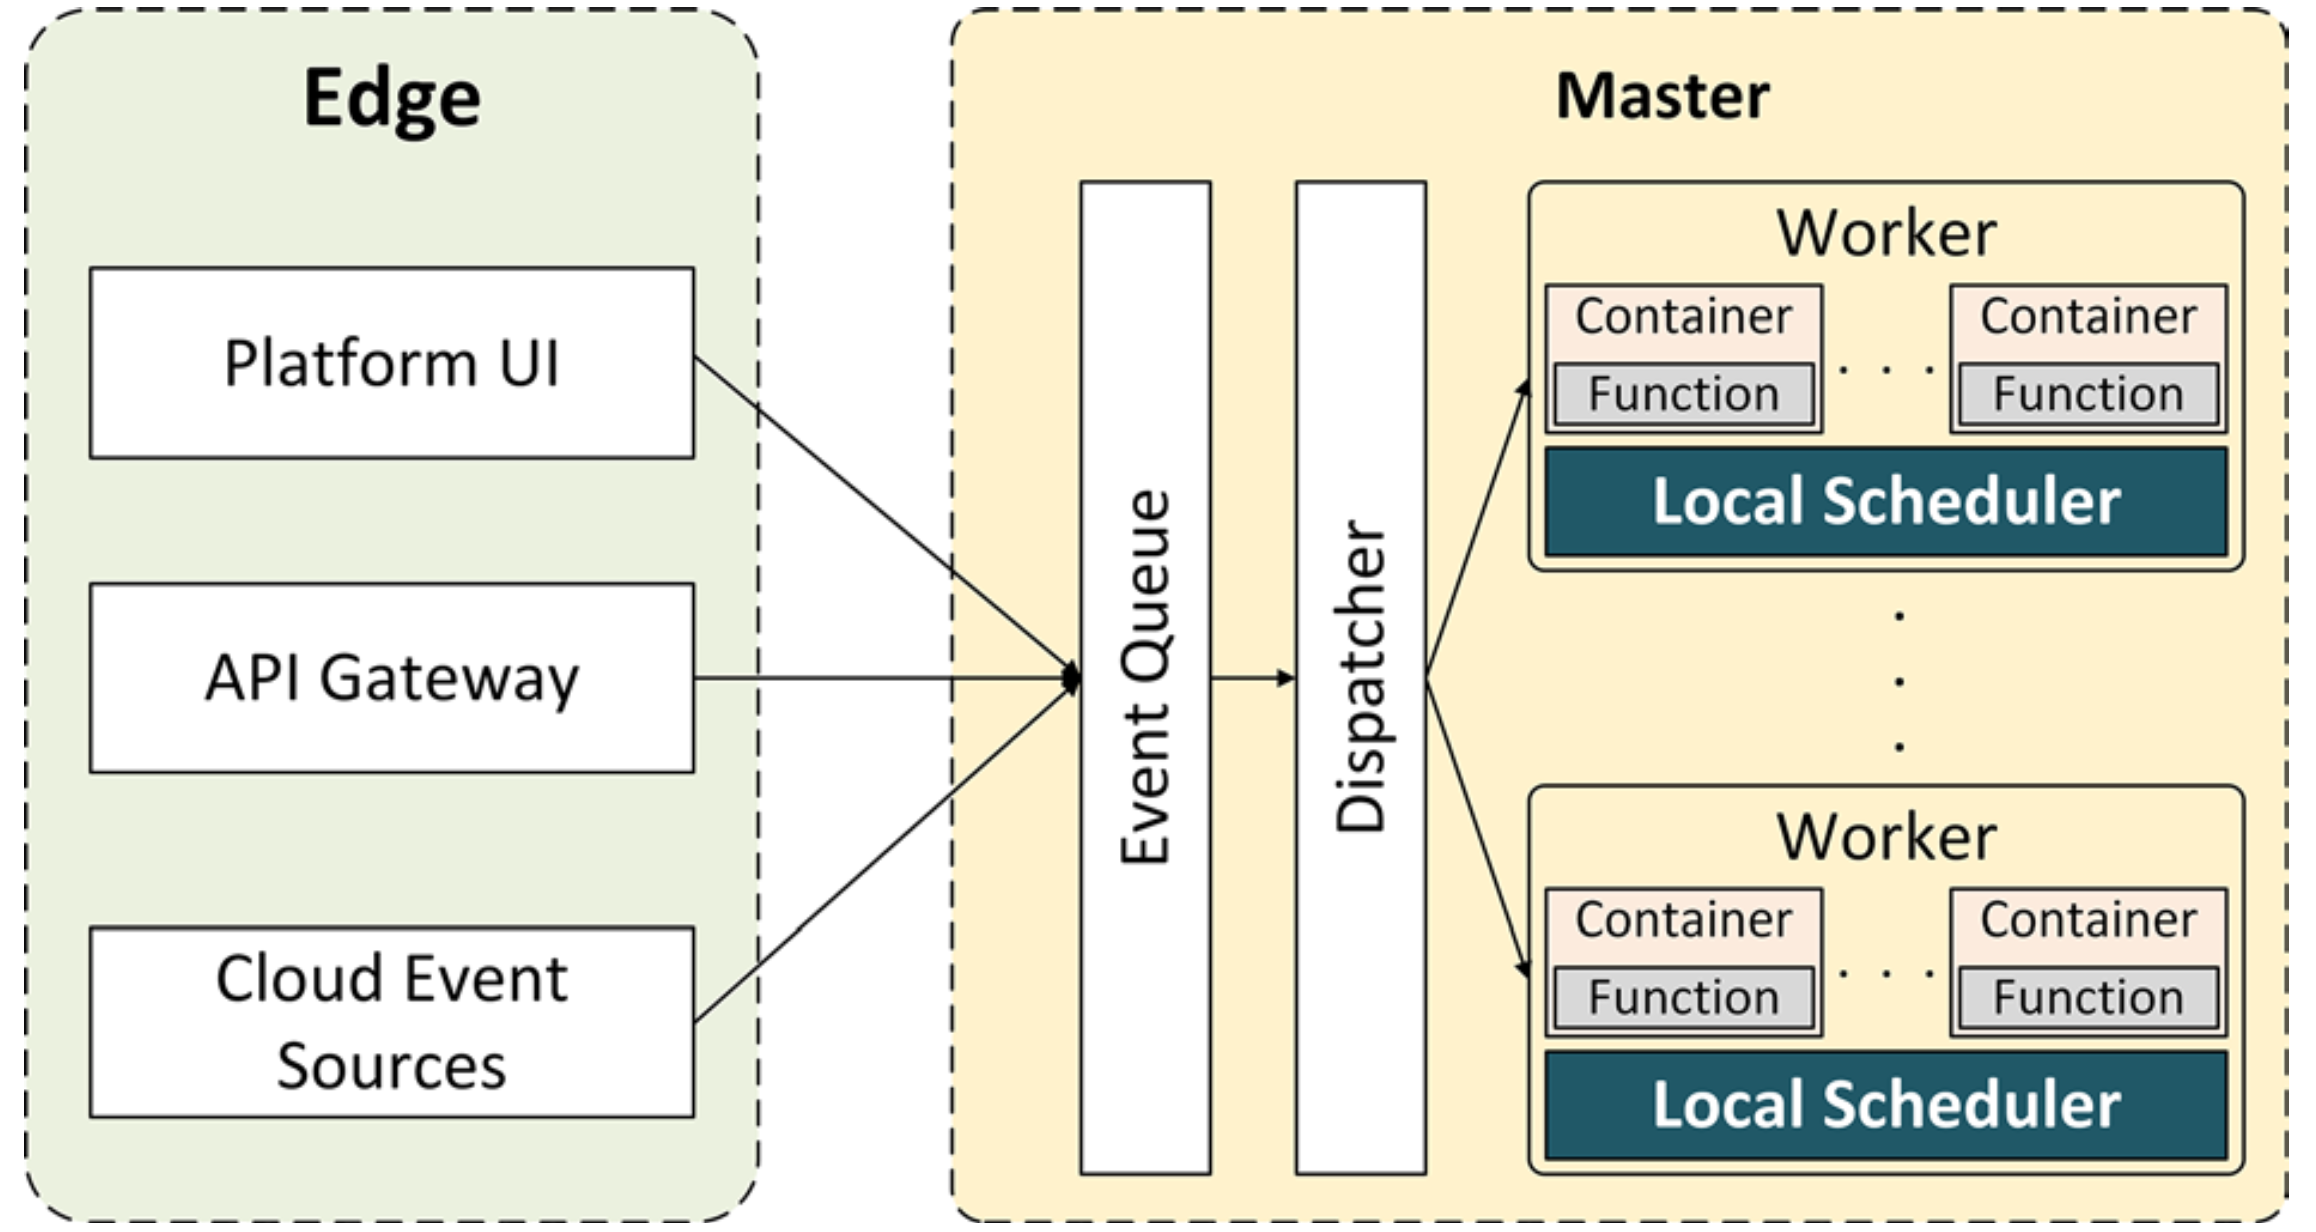
\includegraphics[width=0.7\textwidth]{img/arch.png}
    \captionof{figure}{Blueprint of serverless platform architecture}
    \vspace{10pt}
\end{center}
A smart load balancer helps prevent workers from becoming overloaded. However, under high invocation rates or sudden bursts, a long execution queue can lead to significant wait times. Additionally, when resources are optimized to use the fewest nodes, some functions may experience delays, affecting \textbf{Quality of Service} (\textbf{QoS}). Consequently, the local scheduling approach plays a critical role in optimizing average function wait times, throughput, and resource utilization at worker nodes.\vspace{14pt}\\
Starting a new instance requires initializing the container with necessary libraries, which can introduce startup latency -- commonly known as a \textbf{cold start}. To reduce cold start delays, cloud providers often keep instances paused after use so they can be quickly reused for future invocations. After a function completes or reaches its maximum execution time, the worker node collects execution logs and makes the results available to the user. Scale-to-zero functionality allows users to pay only for the exact time and resources used during active function execution.\cite{banaei2022etas}

\section{Apache Openwhisk}
Apache Openwhisk is an \textbf{open-source serverless} platform created by \textbf{IBM} that executes functions in response to events, scaling automatically and managing all necessary infrastructure and services. OpenWhisk competes with large platforms like \textit{Nginx}, \textit{Kafka}, \textit{Docker}, and \textit{CouchDB}; together, these tools help create a comprehensive serverless cloud service.\vspace{14pt}\\
It’s commonly used for applications that need \textbf{flexibility}, \textbf{scalability}, and \textbf{agility}, especially where real-time processing or dynamic scaling is important. Some pratical scenarios where Openwhisk shines are \textit{Real-Time Data Processing}, \textit{IoT Data Processing}, \textit{Automated DevOps Tasks} and \textit{Serverless API Backend}.\vspace{14pt}\\
Additionally, OpenWhisk provides a \textit{Command Line Interface} (\textit{CLI}), known as \textbf{wsk}, which allows developers to easily create, execute, and manage OpenWhisk entities across any operating system, making platform interactions straightforward for developers.\vspace{14pt}\\
Apache Openwhisk supports flexible deployment options across various platforms due to its containerized components, which enable deployment both locally and within cloud infrastructures. It can be deployed on platforms such as \textit{Kubernetes}, \textit{Mesos}, and \textit{OpenShift}.\vspace{14pt}\\
The programming model of Apache Openwhisk is built around three core components:\\
\textit{Actions}, \textit{Triggers}, and \textit{Rules}.\vspace{14pt}\\
\textbf{Actions} are stateless functions that execute arbitrary code; \textbf{Triggers} represent a class of events originating from various sources, and \textbf{Rules} link a Trigger to an Action. OpenWhisk also allows chaining Actions into sequences.\vspace{14pt}\\
The model supports multiple programming languages, including \textit{Java}, \textit{Python}, and \textit{JavaScript}, and uses an event-driven architecture where most \textbf{Actions execute in response to events}.\cite{quevedo2019evaluating}\vspace{10pt}
\begin{center}
    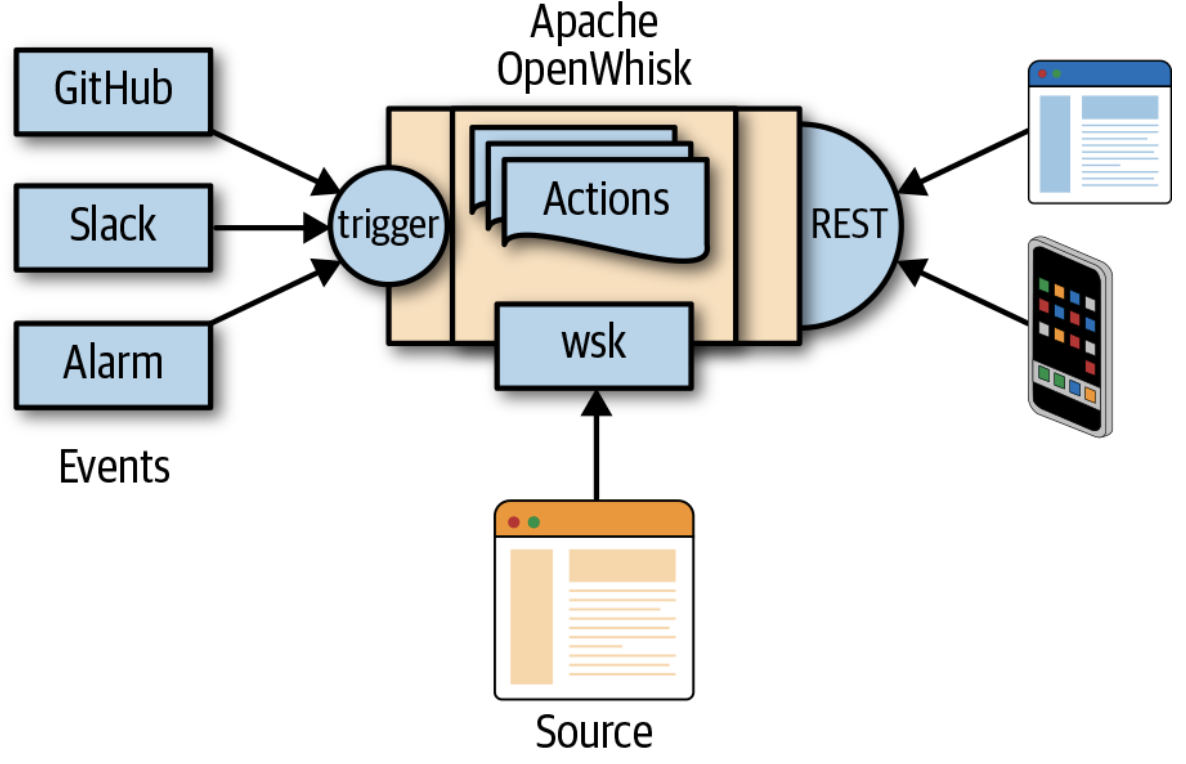
\includegraphics[width=0.7\textwidth]{img/ow_works.png}
    \captionof{figure}{How Apache Openwhisk works}
    \vspace{10pt}
\end{center}
In summary, this platform’s key features include\cite{huy2021crypto}:
\begin{itemize}
    \item \textbf{Deploys Anywhere}: with its container-based architecture, Apache Openwhisk offers versatile deployment options, supporting both local setups and various cloud infrastructures.
    \item \textbf{Supports Any Programming Language}: OpenWhisk is compatible with a wide range of programming languages, including NodeJS, Java, Scala, PHP, Python, and others. For unsupported platforms or languages, users can easily create and customize executables using Docker SDK to run on Docker.
    \item \textbf{Integration Support}: OpenWhisk enables easy integration of developed Actions with popular services through pre-built packages, either from independent projects or the default catalog. These packages offer integrations with services such as Kafka message queues, databases, mobile applications, messaging services, and RSS feeds.
    \item \textbf{Rich Function Composition}: functions written in multiple programming languages can be packaged with Docker for flexible invocation options, including synchronous, asynchronous, or scheduled execution. Parameter binding is recommended to prevent hardcoding service credentials directly into code.
    \item \textbf{Scalability and Resource Optimization}: OpenWhisk allows Actions to scale instantly, handling thousands of executions in seconds or running only as needed, such as on a weekly schedule. Resources scale automatically to match demand, pausing when idle, so users only pay for actual usage with no costs for unused resources.
\end{itemize}

\section{Apache Openwhisk Main Architectural Drivers}
Apache Openwhisk’s architecture is shaped by several key non-functional requirements that are essential for delivering a \textit{scalable}, \textit{flexible}, and \textit{reliable} Function-as-a-Service (FaaS) platform. These architectural drivers address the \textit{performance}, \textit{scalability}, \textit{flexibility}, \textit{reliability}, \textit{security}, and \textit{ease of use} demanded in serverless environments.\\
Below is an overview of the main architectural drivers and their impact on Openwhisk’s design.
\subsection{Scalability and Elasticity}
One of the primary drivers for any FaaS platform is the ability to \textbf{scale on-demand} in response to \textbf{workload fluctuations}. In serverless environments, workloads are often highly dynamic, requiring rapid scaling up during peak demand and scaling down to save resources during idle times.\vspace{14pt}\\
To support elasticity, Openwhisk’s architecture includes components like an \textbf{Activation Dispatcher}, which manages and routes incoming function requests, and an \textbf{Invocation Controller}, which schedules these functions onto available resources.\\
Openwhisk supports stateless function execution, which allows multiple instances to scale in parallel across distributed nodes without dependencies. The use of container-based isolation (e.g., \textit{Docker} or \textit{Podman}) also enables fast provisioning of resources, which is essential for maintaining high scalability.
\subsection{Low Latency and Fast Cold Start Times}
In serverless architectures, the platform needs to handle sporadic or unpredictable workloads, which often leads to \textit{cold starts} -- instances where containers are launched from scratch due to inactivity. Low latency in handling requests, both during cold starts and for warm containers, is critical to ensuring a responsive user experience.\vspace{14pt}\\
Openwhisk uses a \textbf{pre-warming strategy} where a pool of containers remains active to handle requests immediately, reducing latency from cold starts. Furthermore, the system uses a stateless design for function execution, allowing resources to be quickly reused across requests. This architectural choice \textbf{minimizes the overhead} of setting up new containers, thus achieving \textbf{faster response times even under high concurrency}.
\subsection{Fault Tolerance and Reliability}
Fault tolerance is essential to ensure that the platform can \textbf{handle failures} without impacting the overall service availability. In a distributed, event-driven environment, functions must be resilient to network, hardware, and software failures.\vspace{14pt}\\
Openwhisk’s architecture is designed to distribute functions across \textbf{multiple nodes}, allowing \textit{redundancy} and \textit{failover capabilities}. The platform’s messaging backbone, typically implemented with \textit{Apache Kafka}, supports high-availability messaging and enables reliable event-driven processing.\\
Additionally, Openwhisk includes \textbf{retry mechanisms} for function invocations and provides error-handling configurations that enable applications to recover gracefully from failures.
\subsection{Multi-Tenancy and Isolation}
Multi-tenancy is an essential feature for serverless platforms used by \textbf{multiple users or teams}, requiring isolation to prevent cross-tenant interference or security risks. Proper isolation is also critical to ensure that a high workload from one user does not negatively impact others.\vspace{14pt}\\
Openwhisk uses \textbf{container-based isolation} to execute functions in separate containers, ensuring that the memory, processing, and storage of one function do not affect others. Additionally, Openwhisk includes resource limits and quotas per user or namespace, which helps enforce isolation and control resource usage across tenants. This architecture not only protects user functions but also maintains predictable performance across multiple concurrent workloads.
\subsection{Extensibility and Customizability}
Open-source platforms like Openwhisk aim to be flexible enough to \textbf{support various deployment scenarios}, \textbf{languages}, and \textbf{runtimes}. Extensibility allows organizations to tailor the platform to their specific needs and integrate with different cloud providers or on-premises environments.\vspace{14pt}\\
Openwhisk’s open-source, modular architecture allows developers to add custom runtimes, modify the scheduling logic, or extend the platform’s capabilities with additional services. Openwhisk \textbf{supports various languages out-of-the-box} (such as JavaScript, Python, and Swift), and its plug-and-play nature lets users develop \textbf{custom runtimes} as needed. This extensibility is a key driver for Openwhisk’s popularity in hybrid or private cloud deployments, as it enables full control and customizability to meet organizational needs.
\subsection{Security and Compliance}
Security is a primary concern in any multi-tenant environment, where data \textit{confidentiality}, \textit{access control}, and \textit{isolation} are critical. Compliance with data protection standards (e.g., GDPR, HIPAA) is also often required, especially for enterprises handling sensitive data.\vspace{14pt}\\
Openwhisk includes robust security features, such as \textbf{API authentication}, \textbf{role-based access control}, and \textbf{encrypted communications} between services. By running functions in isolated containers, Openwhisk minimizes the risk of unauthorized access between functions. Additionally, as an open-source project, Openwhisk allows users to implement and audit additional security measures in compliance with organizational and industry standards.
\subsection{Observability and Monitoring}
Observability is essential for maintaining high availability and performance in serverless platforms, especially given the ephemeral nature of FaaS functions. Monitoring tools are needed to gain insights into function execution, detect failures, and optimize performance.\vspace{14pt}\\
Openwhisk includes \textbf{logging and monitoring capabilities}, enabling users to track function execution, resource usage, and latency. By integrating with external monitoring tools like \textit{Grafana} and \textit{Prometheus}, Openwhisk supports comprehensive observability. Furthermore, the platform’s event-driven nature allows it to capture detailed traces of function invocations, which helps in debugging and optimizing application performance.
\vspace{20pt}\\
These architectural drivers form the foundation of Apache Openwhisk’s design and differentiate it in the competitive landscape. By prioritizing \textit{scalability}, \textit{low latency}, \textit{fault tolerance}, \textit{multi-tenancy}, \textit{extensibility}, \textit{security}, and \textit{observability}, Openwhisk provides a robust, customizable, and reliable serverless platform that can adapt to a wide variety of deployment scenarios and workload requirements.\vspace{14pt}\\
These drivers are central to Openwhisk’s appeal as an open-source, vendor-agnostic FaaS solution suitable for both cloud-native and hybrid environments.

\section{Apache Openwhisk Architecture}
Fig. 3 shows the architecture of \textit{Apache Openwhisk}, which consists of two primary components: the \textbf{Controller} and the \textbf{Invoker}, built on \textbf{Nginx}, \textbf{Kafka}, \textbf{Docker}, and \textbf{CouchDB}. Together, these components enable Openwhisk to function as a \textit{serverless event-driven programming service}. Openwhisk offers a \textit{RESTful API} that allows users to submit functions and retrieve execution results.\vspace{10pt}
\begin{center}
    \includegraphics[width=0.6\textwidth]{img/ow_arch.png}
    \captionof{figure}{Apache Openwhisk architecture}
    \vspace{10pt}
\end{center}
\textbf{Nginx} routes incoming requests to the \textit{Controller}, which handles authentication, retrieves the requested functions from the \textbf{CouchDB} database, and directs them to the \textit{Invokers} acting as a \textit{Load Balancer}.\vspace{14pt}\\
\textbf{Kafka}, a high-performance message distribution system, facilitates communication between the \textit{Controller} and the \textit{Invokers}.\vspace{14pt}\\
The \textit{Invokers}, distributed across multiple machines and responsible for hosting serverless function containers, execute function calls by allocating resources within \textbf{Docker} containers and assigning a container to each function invocation. Essentially, \textit{Invokers} serve as the \textit{worker nodes} in Openwhisk (as represented in Fig. 1).\vspace{14pt}\\
Each \textit{Invoker} has an in-memory queue to manage function requests when resources are temporarily unavailable. Once resources are freed, functions are dequeued and executed in a \textbf{First Come First Serve} (\textbf{FCFS}) order. All \textit{Invokers} use the same instructions embedded in the \textit{Invoker component's source code} (written in \textit{Scala}), ensuring uniform operation across all \textit{Invokers}.\vspace{14pt}\\
Users can register on the platform to upload their functions, specifying only the memory required for each function's execution.\cite{banaei2022etas}\vspace{14pt}\\
Fig. 4 shows how Openwhisk processes an action into more details.\cite{sciabarra2019learning}\vspace{10pt}
\begin{center}
    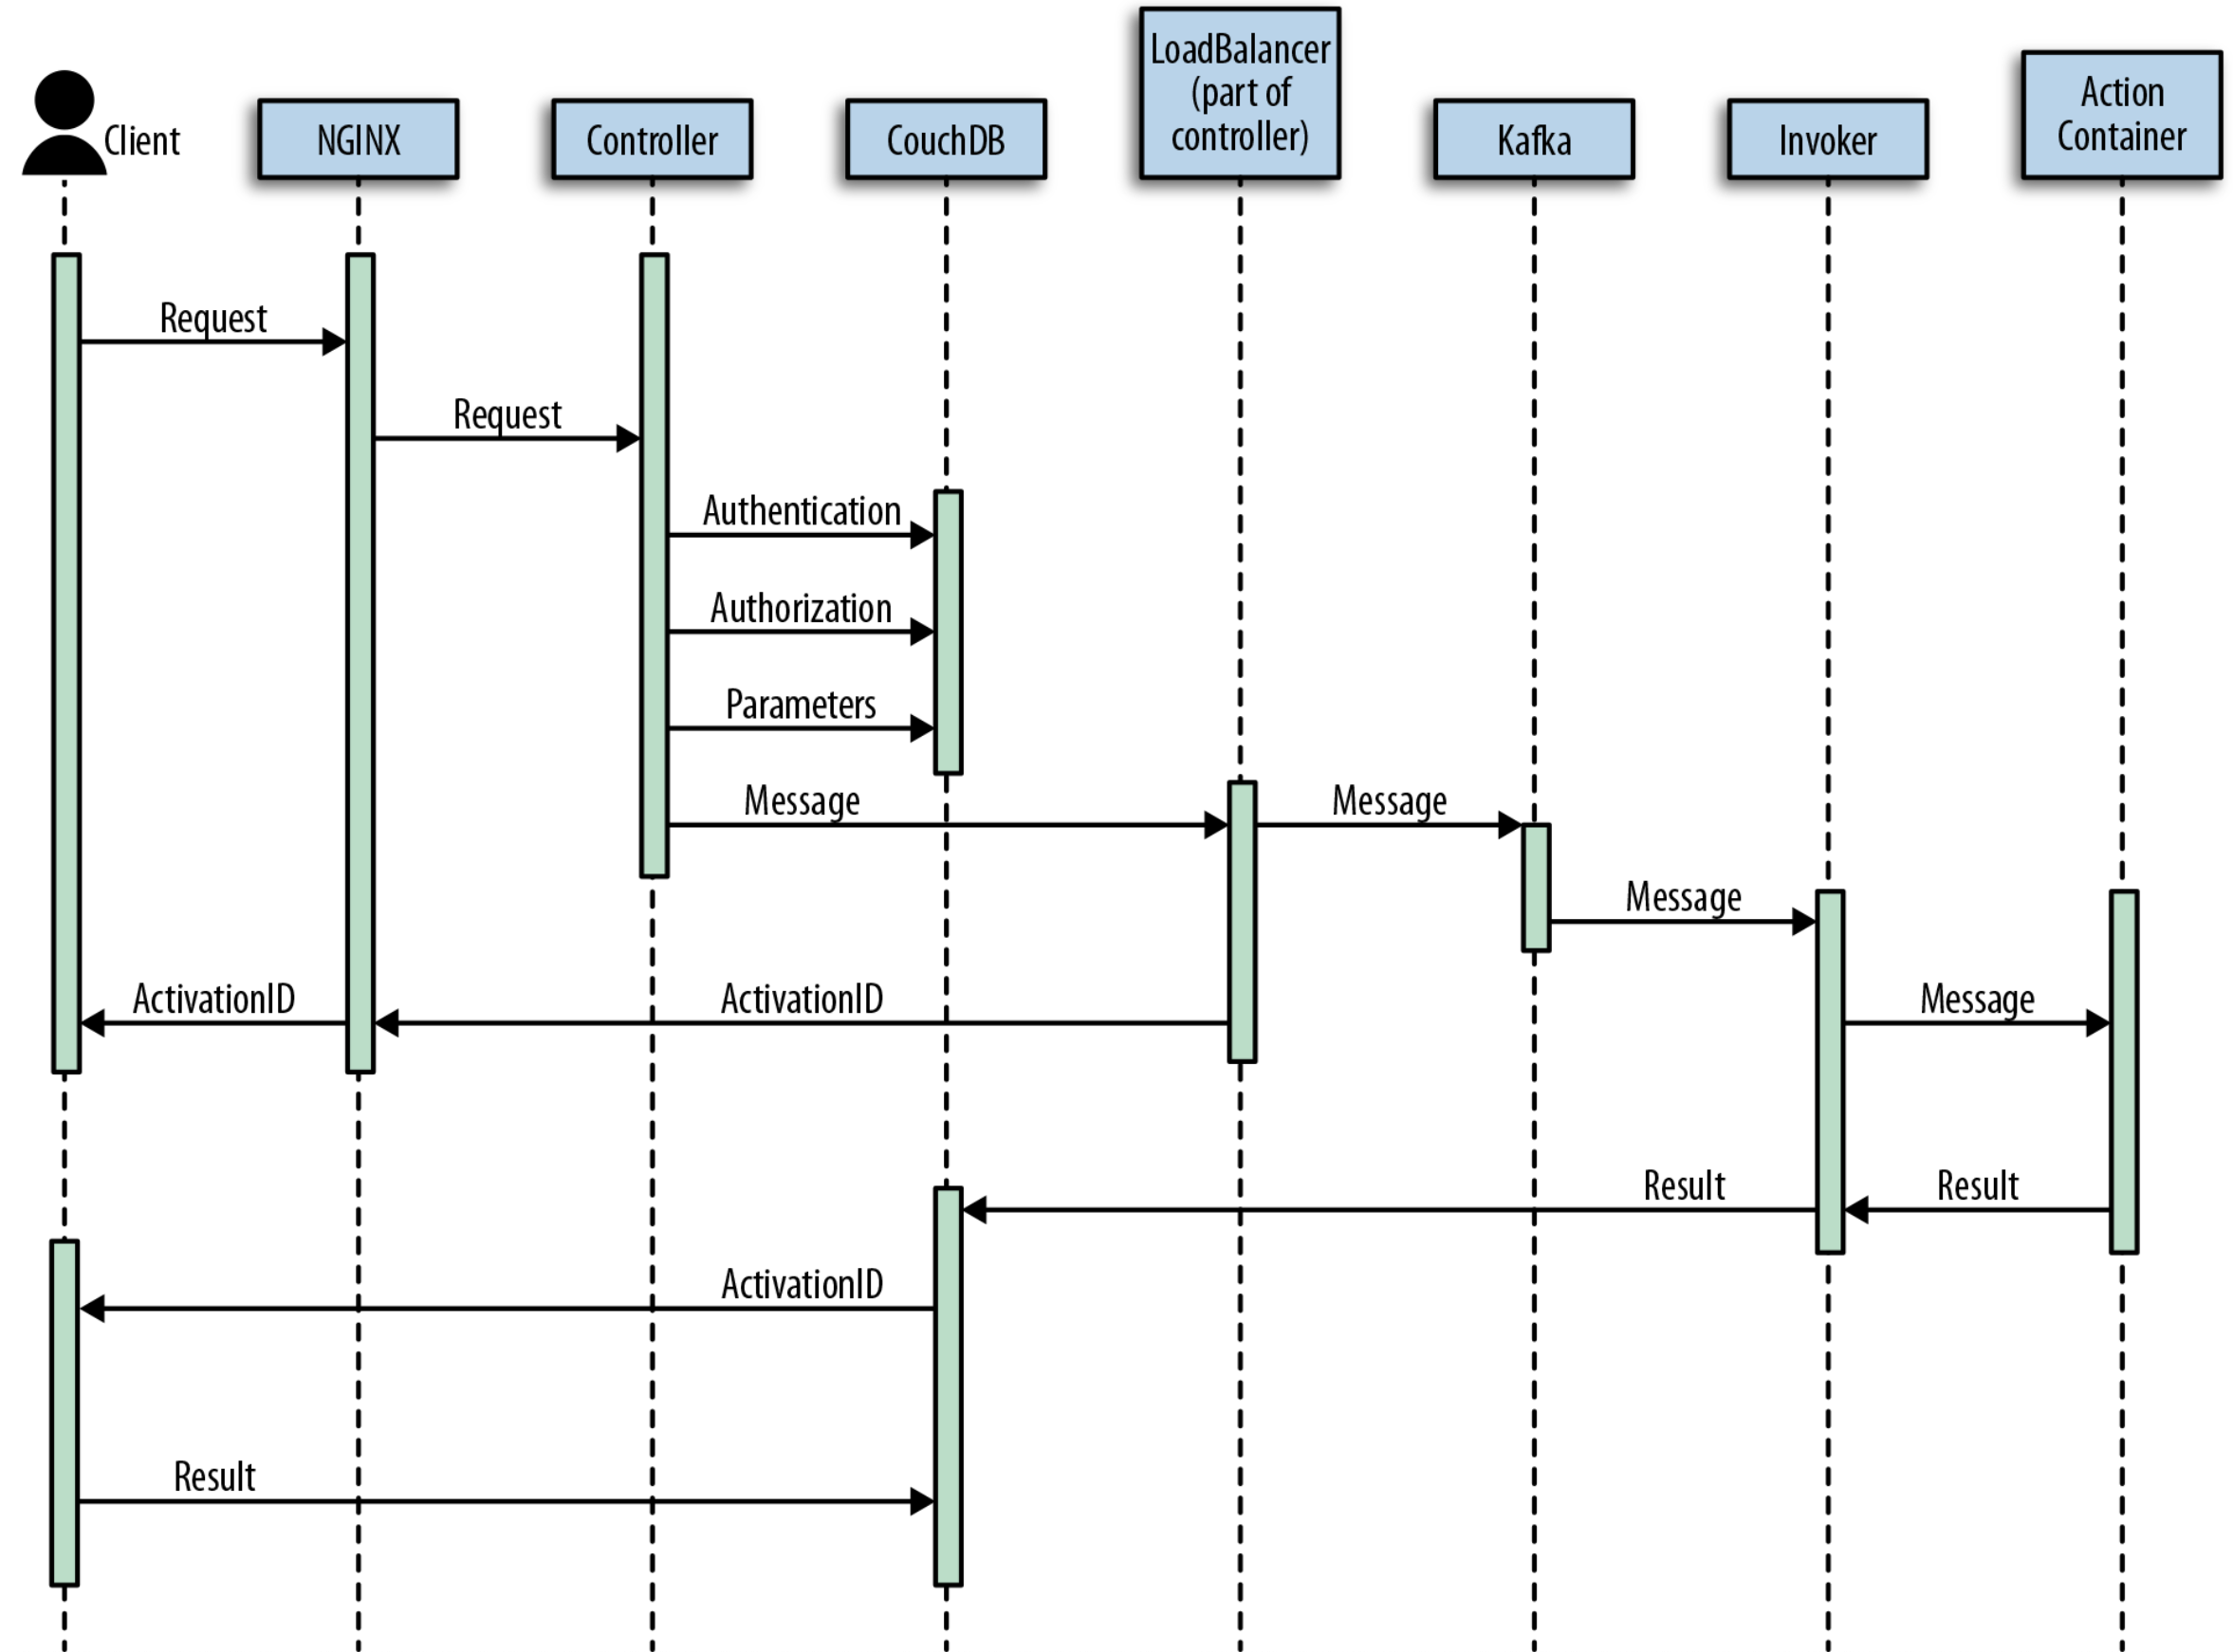
\includegraphics[width=0.95\textwidth]{img/sequence.png}
    \captionof{figure}{How Openwhisk processes an action}
    \vspace{10pt}
\end{center}
\textbf{Nginx}\\
The process begins when an action is invoked, which can happen in several ways:
\begin{itemize}
    \item Via the web, if the action is set up as a web-accessible action.
    \item Through the API, when one action calls another.
    \item By activating a trigger with a rule linked to the action.
    \item From the CLI (Command Line Interface).
\end{itemize}
The \textit{client} refers to the entity initiating the action. As Openwhisk is a RESTful system, each invocation is translated into an HTTPS request that first reaches the \textit{edge} node. This edge node is the web server and reverse proxy, Nginx.\\
Nginx’s primary function here is to handle HTTPS, deploying the necessary certificates for secure processing.\\
Once secure, Nginx forwards the request to the system's core service component, the Controller.\vspace{70pt}\\
\textbf{Controller}\\
Before executing an action, the controller verifies that the action can be properly executed and initialized:
\begin{itemize}
    \item \textbf{Authentication}: the controller must first authenticate the request to confirm it can execute the action.
    \item \textbf{Authorization}: after confirming the request’s origin, the controller checks that the client has the necessary permissions to proceed.
    \item \textbf{Parameter Enrichment}: the request is then supplemented with additional parameters that are part of the action’s configuration.
\end{itemize}
To carry out these steps, the controller consults CouchDB, the database used by Openwhisk. Once the request is validated and enriched, the action is ready for execution and is sent to the load balancer, the next step in the processing flow.\vspace{14pt}\\
\textbf{Load Balancer}\\
The Load Balancer in Openwhisk is responsible for distributing the processing load across various executors, known as Invokers.\\
Since Openwhisk runs actions within designated runtimes, the load balancer tracks available runtime instances. When possible, it reuses existing instances to execute actions; if not, it creates new instances as needed.\vspace{14pt}\\
When the system is ready to invoke an action, the load balancer can't send requests directly to an invoker if it is already occupied, has crashed, or if the system is undergoing a restart. Operating in a highly parallel, scalable environment means the system may not always have immediate resources available, necessitating a buffer for pending invocations. Openwhisk uses Kafka for this buffering.\vspace{14pt}\\
Kafka, a high-performance \textit{publish and subscribe} messaging system, stores requests until they are ready for execution. Each action invocation is converted into an HTTPS request to Nginx, which is then transformed into a Kafka message directed to the chosen invoker.\\
Each message assigned to an invoker includes a unique identifier, the activation ID. Once queued in Kafka, the system offers two types of invocation responses:
\begin{itemize}
    \item \textbf{Nonblocking Invocation}: the activation ID is immediately returned to the client as the response, completing the request. The client can later use this ID to retrieve the invocation result.
    \item \textbf{Blocking Invocation}: the connection remains open as the controller waits for the action to complete. Once the result is ready, it is sent directly to the client.
\end{itemize}
\vspace{5pt}
\textbf{Invoker}\\
In Openwhisk, the invoker is responsible for executing actions within isolated environments provided by Docker containers. Docker containers simulate a complete operating system, offering a self-contained environment with all dependencies needed to run an action.\vspace{14pt}\\
From the action’s viewpoint, the Docker container resembles a full computer, similar to a virtual machine (VM), but container execution is significantly more efficient than VMs, making containers the preferred choice.\\
Docker uses images to create containers for action execution. Each runtime corresponds to a Docker image, and the invoker launches a new image for the specified runtime, then loads the action’s code into it. Openwhisk offers a variety of pre-built Docker images that support different programming languages, including JavaScript, Python, Go, and Java. These images come with initialization logic specific to each runtime.\\
Once the runtime environment is initialized, the invoker processes action requests, handling and storing logs to aid debugging.\vspace{14pt}\\
After the action execution is complete, Openwhisk stores the result in CouchDB (also used for configuration data storage). Each action result is tagged with the activation ID, which was previously provided to the client. This allows the client to retrieve the execution result later by querying CouchDB using the activation ID.\vspace{14pt}\\
\textbf{Client}\\
The processing flow in Openwhisk is primarily asynchronous. In this mode, the client initiates a request and receives an activation ID, which acts as a reference for the invocation. This activation ID allows Openwhisk to store the result of the action in the database upon completion. To retrieve the final result, the client must send another request later, using the activation ID as a parameter. Once the action finishes, the result, logs, and additional information are stored in the database, making them accessible for the client.\vspace{14pt}\\
Openwhisk also supports synchronous processing, which operates similarly but with one key difference: the client’s request remains open, blocking until the action completes, allowing the client to immediately receive the result.\cite{sciabarra2019learning}

\section{Competing solutions}
Apache Openwhisk is one of many solutions in the rapidly evolving serverless and Function-as-a-Service (FaaS) ecosystem. It competes with several other platforms, each offering distinct features, operational models, and deployment options.\vspace{14pt}\\
Notable competitors include \textit{Amazon Web Services} (\textit{AWS}) \textit{Lambda}, \textit{Google Cloud Functions} and \textit{Microsoft Azure Functions}.\\
Below is an overview of how these solutions compare with Apache Openwhisk in terms of \textit{functionality}, \textit{scalability}, \textit{ecosystem integration}, and \textit{operational control}.
\subsection{AWS Lambda}
\textbf{AWS Lambda}, launched in 2014 by \textbf{Amazon Web Services}, was the first mainstream FaaS platform and remains a leader in the market. AWS Lambda enables users to run code in response to events without managing servers.\vspace{14pt}\\
\textbf{Strengths}: Lambda offers seamless integration with AWS’s extensive suite of services, which makes it highly appealing for users already in the AWS ecosystem. Its developer tooling and monitoring support are advanced, with options for logging, tracing, and error handling through services like Amazon CloudWatch and X-Ray.\vspace{14pt}\\
\textbf{Weaknesses}: Lambda is closely tied to the AWS ecosystem, and migrating workloads to or from AWS can involve considerable re-architecture. Additionally, Lambda’s default runtime has a cold start latency, which can affect performance for latency-sensitive applications.\vspace{14pt}\\
\textbf{Comparison with Openwhisk}: while AWS Lambda excels in native AWS integration and scalability, Openwhisk offers a more flexible deployment model, allowing for cloud, hybrid, or on-premises installations, which is ideal for users with strict data locality requirements or those operating in multi-cloud environments.
\subsection{Google Cloud Functions}
\textbf{Google Cloud Functions} (\textbf{GCF}) provides an event-driven serverless compute service on \textbf{Google Cloud Platform}. It supports multiple languages, including Node.js, Python, and Go.\vspace{14pt}\\
\textbf{Strengths}: GCF is tightly integrated with GCP services, including Google Cloud Pub/Sub, Google Firestore, and Firebase. It is known for rapid auto-scaling and has low latency due to Google’s extensive global network infrastructure.\vspace{14pt}\\
\textbf{Weaknesses}: like Lambda, GCF’s integration primarily focuses on GCP, making it less flexible for users with multi-cloud requirements. Cold start times, although improved, remain a concern in certain use cases.\vspace{14pt}\\
\textbf{Comparison with Openwhisk}: GCF is highly performant within the Google ecosystem but lacks the deployment flexibility that Openwhisk provides. Openwhisk’s open-source model allows for higher customization and control, while GCF is a managed solution with limited customization.
\subsection{Microsoft Azure Functions}
\textbf{Microsoft Azure Functions} is a FaaS solution on the \textbf{Azure Cloud Platform}, supporting a range of programming languages and tight integration with Microsoft’s services like Azure DevOps, Azure Cosmos DB, and Azure Event Grid.\vspace{14pt}\\
\textbf{Strengths}: Azure Functions are well-suited for .NET developers, given Microsoft’s strong support for C\# and Visual Studio integration. The platform is known for its extensive developer tooling, ease of use, and support for both consumption-based and dedicated pricing plans.\vspace{14pt}\\
\textbf{Weaknesses}: Azure Functions, like other proprietary platforms, has limitations around multi-cloud or on-premises deployment. There are also some concerns around cold start latency, though Microsoft offers a premium plan to mitigate this.\vspace{14pt}\\
\textbf{Comparison with Openwhisk}: Azure Functions offers more extensive support for .NET and is tightly integrated with the Azure ecosystem, while Openwhisk is more language-agnostic and portable. Openwhisk’s flexibility for hybrid or on-premises deployment may be more appealing for organizations that require complete control over their serverless environments.\vspace{20pt}\\
Each of these competing solutions has strengths that make them ideal for specific use cases, with choices largely influenced by an organization’s cloud strategy, operational requirements, and existing skill sets. While AWS Lambda, Google Cloud Functions, and Azure Functions offer powerful, managed FaaS options, they may be less flexible for organizations seeking to avoid vendor lock-in or requiring more control over their infrastructure.\vspace{14pt}\\
Apache Openwhisk, as an \textbf{open-source}, \textbf{language-agnostic}, and \textbf{flexible platform}, stands out for users seeking an adaptable, hybrid FaaS solution that can span both cloud and on-premises environments, without the proprietary constraints of fully managed platforms.

\section{Implementation}
Before talking about the implementation itself, I want to define the main objective of this simple implementation. I want to expose an \textbf{HTTP GET endpoint}, which return a simple \textit{Hello World} string. Unfortunately, that's where the simple stuff ends.\vspace{14pt}\\
First of all, I tried to read \textbf{Apache Openwhisk documentation}\footnote{\url{https://openwhisk.apache.org/documentation.html}} to understand more the Openwhisk environment's setup process.\\
After different attempts to make the \textit{Docker} setup work, I even tried the \textit{Java Standalone} version. Nothing was working the way it was supposed to. I even tried deploying everything on different virtual machines, other than my own machine.\vspace{14pt}\\
I then decided to talk with \textit{Prof. Ciancarini} to get a different point of view of the problem. He suggested reaching out to \textit{Michele Sciabarrà}, the author of the book \textbf{Learning Apache OpenWhisk}\footnote{\url{https://www.oreilly.com/library/view/learning-apache-openwhisk/9781492046158/}}, which runs a company that uses Apache Openwhisk as the backbone of their service. The company is called \textbf{Nuvolaris}\footnote{\url{https://www.nuvolaris.io/}}, and it offers a new serverless approach to Kubernetes.\\
While talking with Sciabarrà, he suggested to use their \textit{spin-off} of Openwhisk, called \textbf{Apache OpenServerless}\footnote{\url{https://openserverless.apache.org/}}, which has a simpler way of deploying the Openwhisk core functionalities.\vspace{14pt}\\
Unfortunately, this process will not be any simpler. I had issues related to this process of deployment too. Reading their documentation, the process was similar to the other one, with less dependencies needed.\\
After some days, during which I tried every possible way of making it work, I tried talking directly with the creators of the Apache OpenServerless software. With their help, I managed to get the system to work, and to finally deploy my \textit{"simple"} implementation.\vspace{14pt}\\
Heartfelt thanks go to \textit{Michele Sciabarrà} and his team, for real-time support while debugging the various problems encountered.\\
Also, a big thank you to the \textbf{ADM team}\footnote{\url{https://students.cs.unibo.it/}} -- especially \textit{Emanuele Grasso}. Thanks to his support, I was provided with a virtual machine that met the requirements of OpenServerless and allowed me to perform all the necessary tests. Their work goes beyond this, providing a very useful service for all students in the Computer Science department and beyond.\vspace{14pt}\\
Let's get back to the implementation.\vspace{14pt}\\
Using the \textit{OpenServerless CLI} (\textbf{ops}), I managed to get everything up and running on the virtual machine. I then wrote a really simple \textbf{Python} script, which returns an \textit{Hello World} message:
\begin{lstlisting}[language=python]
def main(args):
    return {"body": "hello world\n"}
\end{lstlisting}
Using the \textit{ops package create test\_dss} command, I created a test package where \textit{actions} can be stored.\vspace{14pt}\\
\textit{ops action create test\_dss/greet script.py --web true} is going to create the action related to the Python script. Using the \textit{--web} flag with a value of \textit{true} or \textit{yes} allows an action to be accessible via \textbf{REST} interface without the need for credentials.\vspace{14pt}\\
To get the URL related to the action, the \textit{ops action get test\_dss/greet --url} command is used. This returns the action HTTP endpoint, ready to be called and tested.\vspace{14pt}\\
An example of this whole execution of commands can be:
\begin{center}
    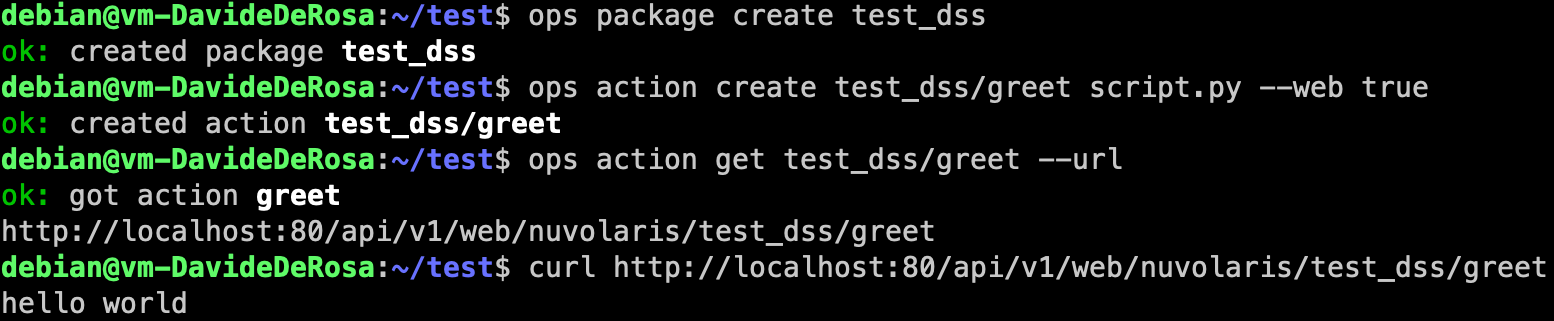
\includegraphics[width=1\textwidth]{img/demo.png}
\end{center}
If you need to update the script, \textit{ops action update test\_dss/greet script.py --web true} is all you need to do.\vspace{14pt}\\
This test shows just the core functionalities of Openwhisk (and OpenServerless). There is a lot more that can be done with this tool. The documentation shows a lot of possible implementations to do, all related to serverless functions.\vspace{14pt}\\
In a possible future study, it would be possible to test Openwhisk performance compared to other Cloud based solution -- like \textit{AWS Lambda} or \textit{Google Cloud Functions}.

\renewcommand{\bibsection}{}
\section*{References}
\bibliography{refs}
\end{document}